\subsection{Fits\-Parallel\-Slices  Class Reference}
\label{class_fitsparallelslices}\index{FitsParallelSlices@{Fits\-Parallel\-Slices}}
Several fits images of the same size to be processed in parallel. 


{\tt \#include $<$fitsslice.h$>$}

Inheritance diagram for Fits\-Parallel\-Slices::\begin{figure}[H]
\begin{center}
\leavevmode
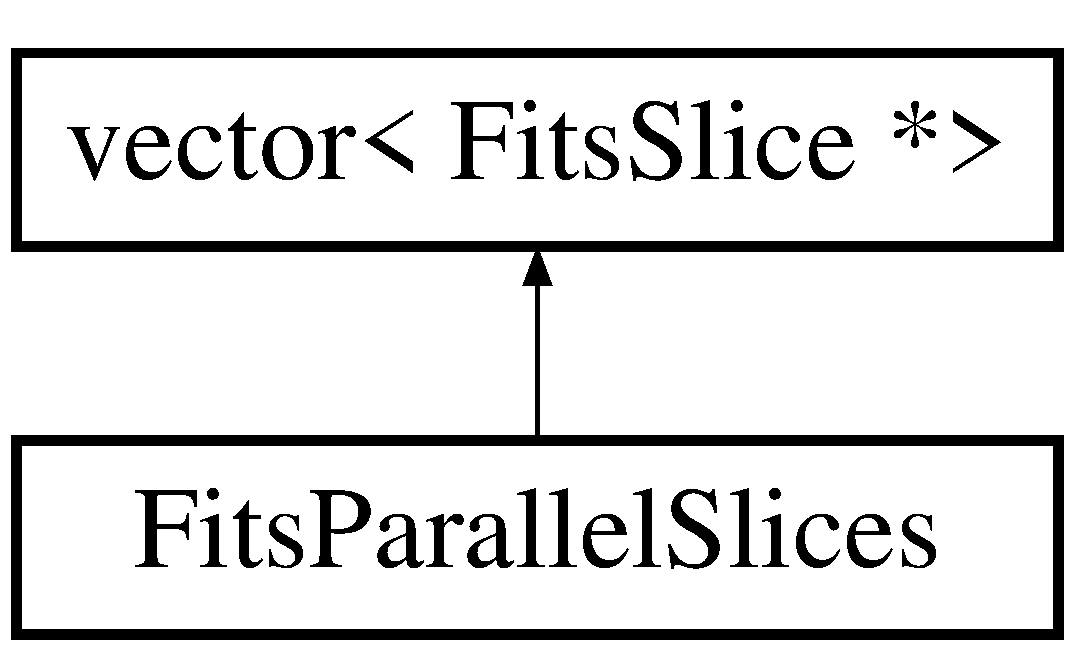
\includegraphics[height=2cm]{class_fitsparallelslices}
\end{center}
\end{figure}
\subsubsection*{Public Methods}
\begin{CompactItemize}
\item 
\index{FitsParallelSlices@{FitsParallelSlices}!FitsParallelSlices@{Fits\-Parallel\-Slices}}\index{FitsParallelSlices@{FitsParallelSlices}!FitsParallelSlices@{Fits\-Parallel\-Slices}}
{\bf Fits\-Parallel\-Slices} (const int Slice\-Size, const int Overlap=0)\label{class_fitsparallelslices_a0}

\begin{CompactList}\small\item\em constructor.\item\end{CompactList}\item 
\index{~FitsParallelSlices@{$\sim$FitsParallelSlices}!FitsParallelSlices@{Fits\-Parallel\-Slices}}\index{FitsParallelSlices@{FitsParallelSlices}!~FitsParallelSlices@{$\sim$Fits\-Parallel\-Slices}}
{\bf $\sim$Fits\-Parallel\-Slices} ()\label{class_fitsparallelslices_a1}

\item 
\index{AddFile@{AddFile}!FitsParallelSlices@{Fits\-Parallel\-Slices}}\index{FitsParallelSlices@{FitsParallelSlices}!AddFile@{Add\-File}}
bool {\bf Add\-File} (const string \&File\-Name)\label{class_fitsparallelslices_a2}

\begin{CompactList}\small\item\em Adds a file in the list. Loads the first slice.\item\end{CompactList}\item 
\index{LoadNextSlice@{LoadNextSlice}!FitsParallelSlices@{Fits\-Parallel\-Slices}}\index{FitsParallelSlices@{FitsParallelSlices}!LoadNextSlice@{Load\-Next\-Slice}}
int {\bf Load\-Next\-Slice} ()\label{class_fitsparallelslices_a3}

\begin{CompactList}\small\item\em load next slice for all involved files. Returns 0 if already on last slice.\item\end{CompactList}\item 
\index{SliceSize@{SliceSize}!FitsParallelSlices@{Fits\-Parallel\-Slices}}\index{FitsParallelSlices@{FitsParallelSlices}!SliceSize@{Slice\-Size}}
int {\bf Slice\-Size} () const\label{class_fitsparallelslices_a4}

\begin{CompactList}\small\item\em size of the current slice size. Different from the constructor value for last slice.\item\end{CompactList}\item 
\index{ImageJ@{ImageJ}!FitsParallelSlices@{Fits\-Parallel\-Slices}}\index{FitsParallelSlices@{FitsParallelSlices}!ImageJ@{Image\-J}}
int {\bf Image\-J} (const int Slice\-J) const\label{class_fitsparallelslices_a5}

\begin{CompactList}\small\item\em return the index in the whole image of the row Slice\-J in the current slice.\item\end{CompactList}\item 
\index{LastSlice@{LastSlice}!FitsParallelSlices@{Fits\-Parallel\-Slices}}\index{FitsParallelSlices@{FitsParallelSlices}!LastSlice@{Last\-Slice}}
bool {\bf Last\-Slice} () const\label{class_fitsparallelslices_a6}

\begin{CompactList}\small\item\em are we in the last slice.\item\end{CompactList}\item 
\index{NFiles@{NFiles}!FitsParallelSlices@{Fits\-Parallel\-Slices}}\index{FitsParallelSlices@{FitsParallelSlices}!NFiles@{NFiles}}
int {\bf NFiles} () const\label{class_fitsparallelslices_a7}

\end{CompactItemize}


\subsubsection{Detailed Description}
Several fits images of the same size to be processed in parallel.

This class is to be used as a handler for {\bf Fits\-Slice} {\rm (p.\,\pageref{class_fitsslice})}'s from files having the same sizes, that one wants to process in parallel (typically to average or sum images). Slices are cut along the second index of the whole image  and have the same size in x as the image.  See {\bf Usage of Fits\-Parallel\-Slices} {\rm (p.\,\pageref{example_slices})} for an example. 



The documentation for this class was generated from the following file:\begin{CompactItemize}
\item 
{\bf fitsslice.h}\end{CompactItemize}
